\documentclass{article}
\usepackage{graphicx}
\usepackage{blindtext}
\usepackage{authblk}
\usepackage{amsmath}
\usepackage{ tipa }
\renewcommand{\familydefault}{\sfdefault}

\title{Statistics 626 - Assignment 03}
\author{Vivek Gupta\thanks{vivek235@tamu.edu}}
\affil{Department of Statistics, Texas A \& M University}



\begin{document}
	\maketitle
	\newpage 


\section{I}

\subsection{a.}
The two random walks $x_t$ , $y_t$ are simulated and shown below in the Figure \ref{fig1:input-series}
These are simulated with initial values of $x_0$ , $y_0$ = 0 , using two independent N(0,1) white noises.

\begin{figure}
	\centering
	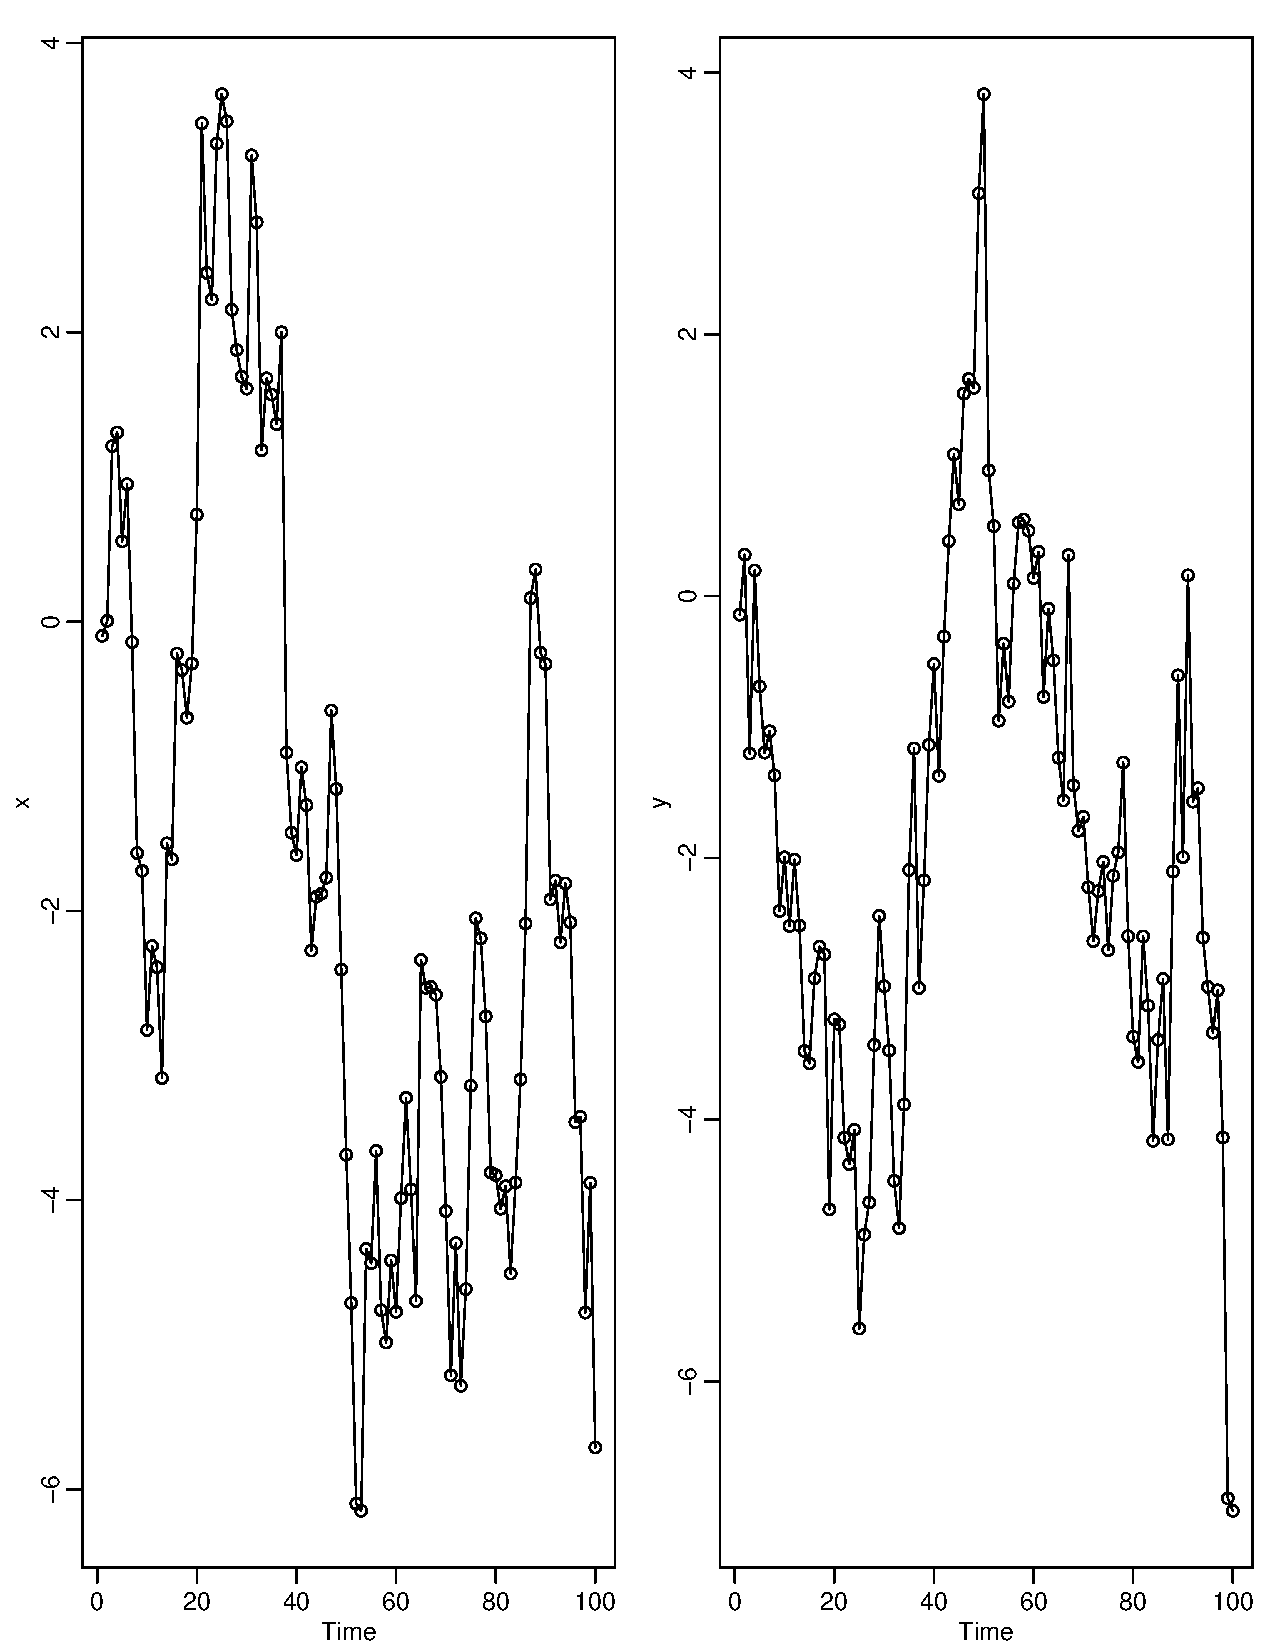
\includegraphics[width=0.9\textwidth]{Parta1}
	\caption{Input series , $y_t$ vs $x_t$}
	\label{fig1:input-series}
\end{figure}

\subsection{i.}

The plots are shown in Figure \ref{fig2:normalplot} and \ref{fig3:lag10}. The first plot shows the lag 0 relationship between series x and y. While the second plot shows 
the relationship between $x_{t-h}$ and $y_t$ at each of the lags from $h$ = 0, 1, 2, 3 ... 10

\begin{figure}
	\centering
	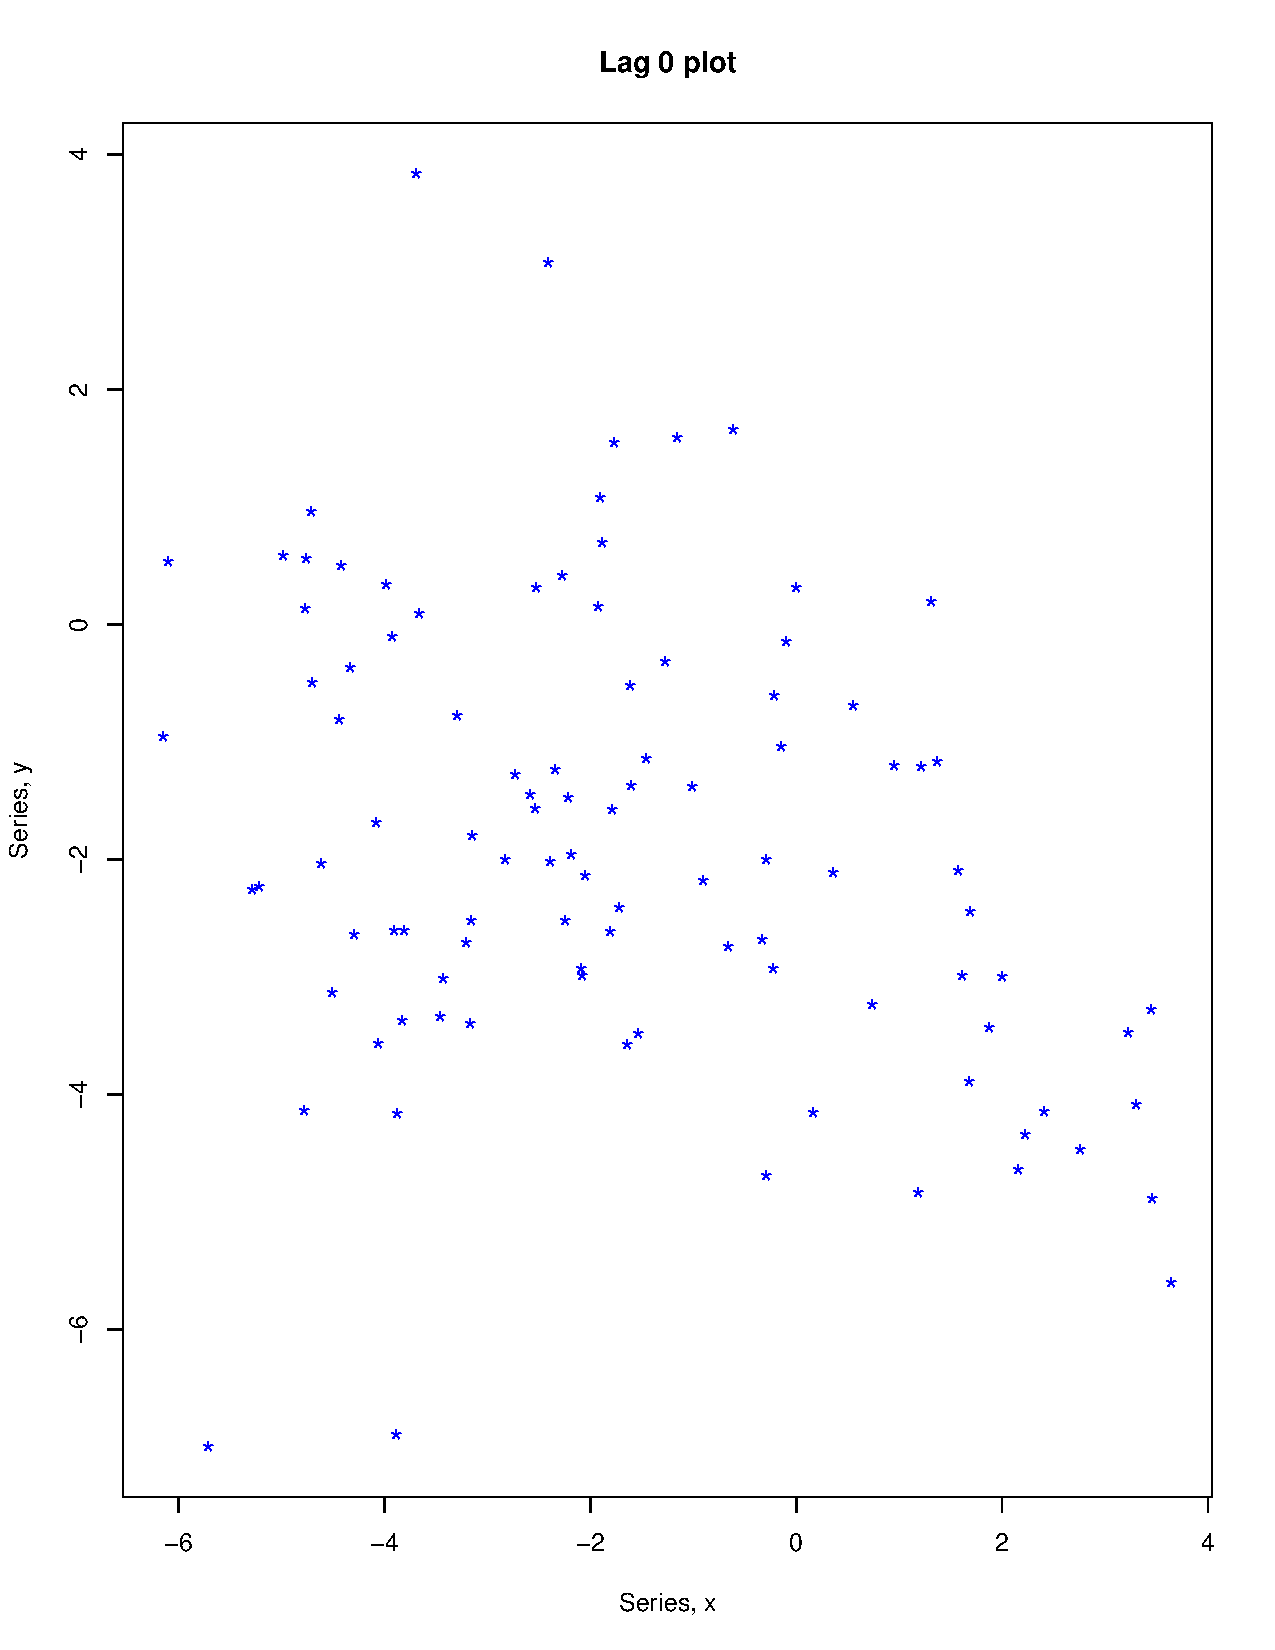
\includegraphics[width=0.9\textwidth]{Lag0}
	\caption{Lag 0 plot , $y_t$ vs $x_t$}
	\label{fig2:normalplot} 
\end{figure}

\begin{figure}
	\centering
	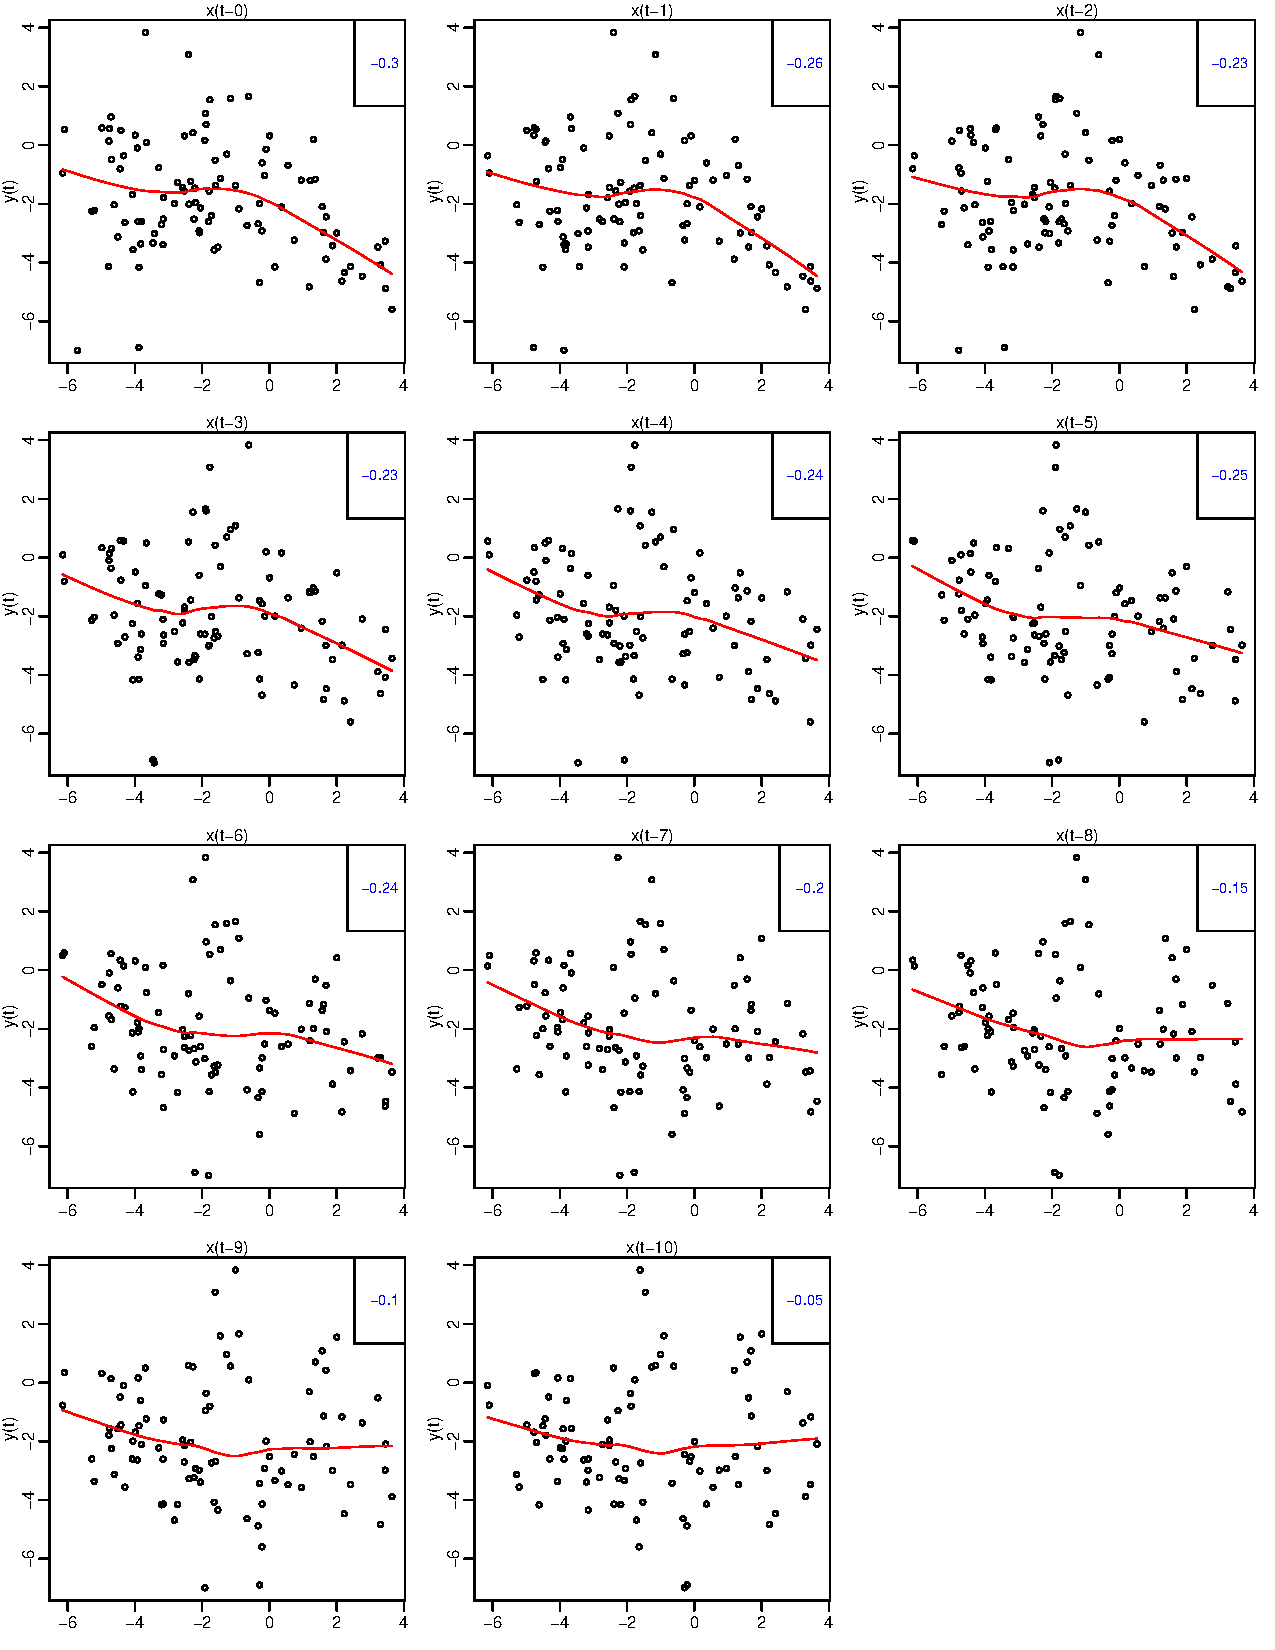
\includegraphics[width=0.9\textwidth]{lagplots_10}
	\caption{Lag $h$ plot , $y_t$ vs $x_{t-h}$}
	\label{fig3:lag10}
\end{figure}
\newpage

We notice some non - linear relationship between the two series as shown in the above figure as is evident from the smoothed fit in each of the graphs. This relationship differs subtly at various lags. At lag valeu $h$ = 9 , 10 we fail to notice any relationship between the two series. 

The correlation coefficient as shown is all less than 0.5 and hence we do not have a very strong linear relationship between these
two series at various values of the lag. 

\subsection{ii.}

Consider the linear regression between $x_t$ and $y_t$ as shown below 


\[
y_t = \beta{_0} + \beta{_1}x_t + w_t
\]

The above, simple linear regression model is valid upon certain constraints or assumptions that $w_t$ is $i.i.d$ N(0,$\sigma^2$)

%We consider the hypothesis , at $\alpha$ = 0.5 \[  H_o : \beta{_1} = 0 , H_1: \beta{_1} \textdoublebarslash  0  \]
But since there isn't a linear relationship as evident from Figure~\ref{fig3:lag10} , we expect to fail to reject the null hypothesis.

\subsection{iii.}

The linear fit summary is shown in Figure \ref{fig4:fit} . The test for \[  H_o : \beta{_1} = 0  \] is significant given the output of the model at a p-value of 0.00237 and \[ \alpha = 0.05 \] . 

When we look at the residual plot as in Figure \ref{fig:Residual-Plot} to diagnose the validity of the model we notice that  
the residuals does not follow the assumption of the model. The residuals vs. the fitted definitely shows a non linear pattern and the residuals do not look to be coming from a normal distribution. Thus, the assumptions of the model are not met with this inear fit.

However, if we assume that the model is valid , then the we have evidence to reject the null hypothesis and conclude that 
at p-value $<$ 0.05, the covariate $x_t$ is significant in explaining the variability in $y_t$.
\begin{figure}
	\centering
	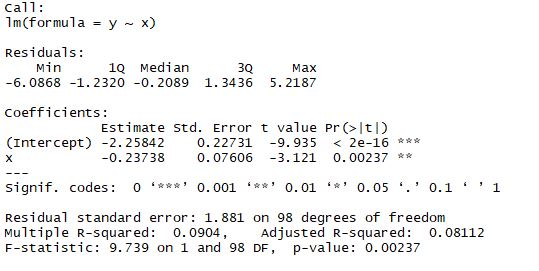
\includegraphics[width=0.9\textwidth]{Fit}
	\caption{Linear fit between $x_t$ , $y_t$ }
    \label{fig4:fit}
\end{figure}

\begin{figure}
	\centering
	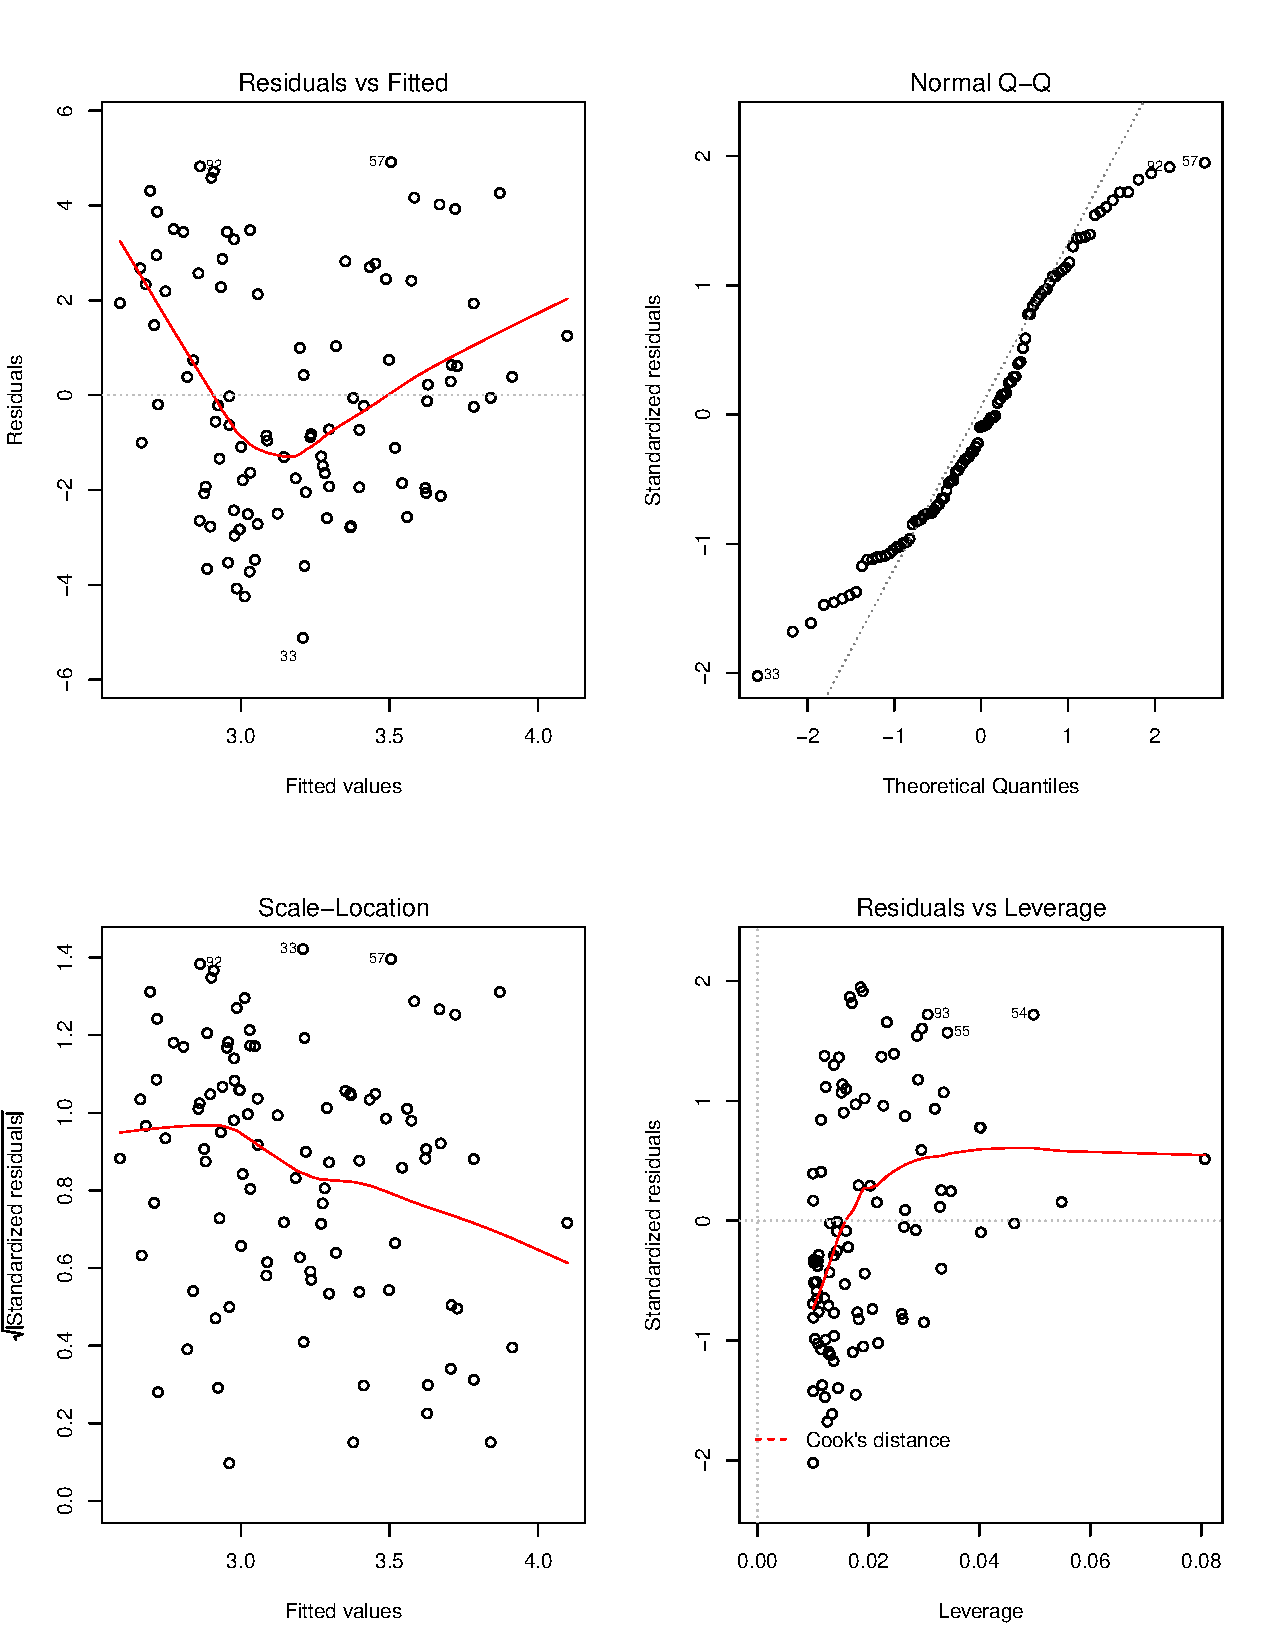
\includegraphics[width=0.9\textwidth]{Residualplot}
	\caption{Residual Plot of the linear fit }
	\label{fig:Residual-Plot}
\end{figure}

\newpage

\subsection{b}

We repeated the above experiment 1000 times and noted that approx. 75 pc. of the times the test concluded that the covariate $x_t$ is significant. 

Clearly this does not support our expectation based on what we noted for the relationship in Figures \ref{fig2:normalplot} and \ref{fig3:lag10} . 

We also has noted earlier based on residual plot shown in Figure. \ref{fig:Residual-Plot} that the model is invalid due to 

\begin{enumerate}
	\item  The relationship between $x_t$ and $y_t$ is non linear.
	\item  Residuals show a pattern of non linearity and thus are not independent. 
	\item  We have evidence of heteroscedasticity in the model.
	\item  Normality in the residuals is questionable. 
\end{enumerate}

Since the model is invalid , the statistical summaries and results such as the p-value of the AOV and significance of the covariate are all invalid and thus the result of linear fit cannot be relied upon.

\newpage

\section{2.6}

\subsection{a}

We can notice the evidence of non homogeneous variances in the varve observations in Figure \ref{fig:tsplot-varve} . We divide the dataset into two equal halves and plot them as shown in the Figure \ref{fig:Density-varve-Plot}.Difference in the variance 
is clearly visible in the two halves of the dataset. We can see the range of the varve varies significantly in the two halves. 

We then take a log transformation of the data to ascertain is the variances are controlled by this mathematical operation.
We notice a pattern emerging out as shown in Figure \ref{fig:tsplot-lvarve}. Further more, the variances in two halves of the 
dataset which were highly variable does not look too much of a problem as shown in Figure \ref{fig:Density-lvarve-Plot}. 
The transformation has greatly aided normality in the data. Figure \ref{fig:QQPlot} shows that the normality has improved. 
It was also noted that the p-value of the Shapiro - Wilk test in the transformed data is 0.016 which still does not indicate a very good fit.

\begin{figure}
	\centering
	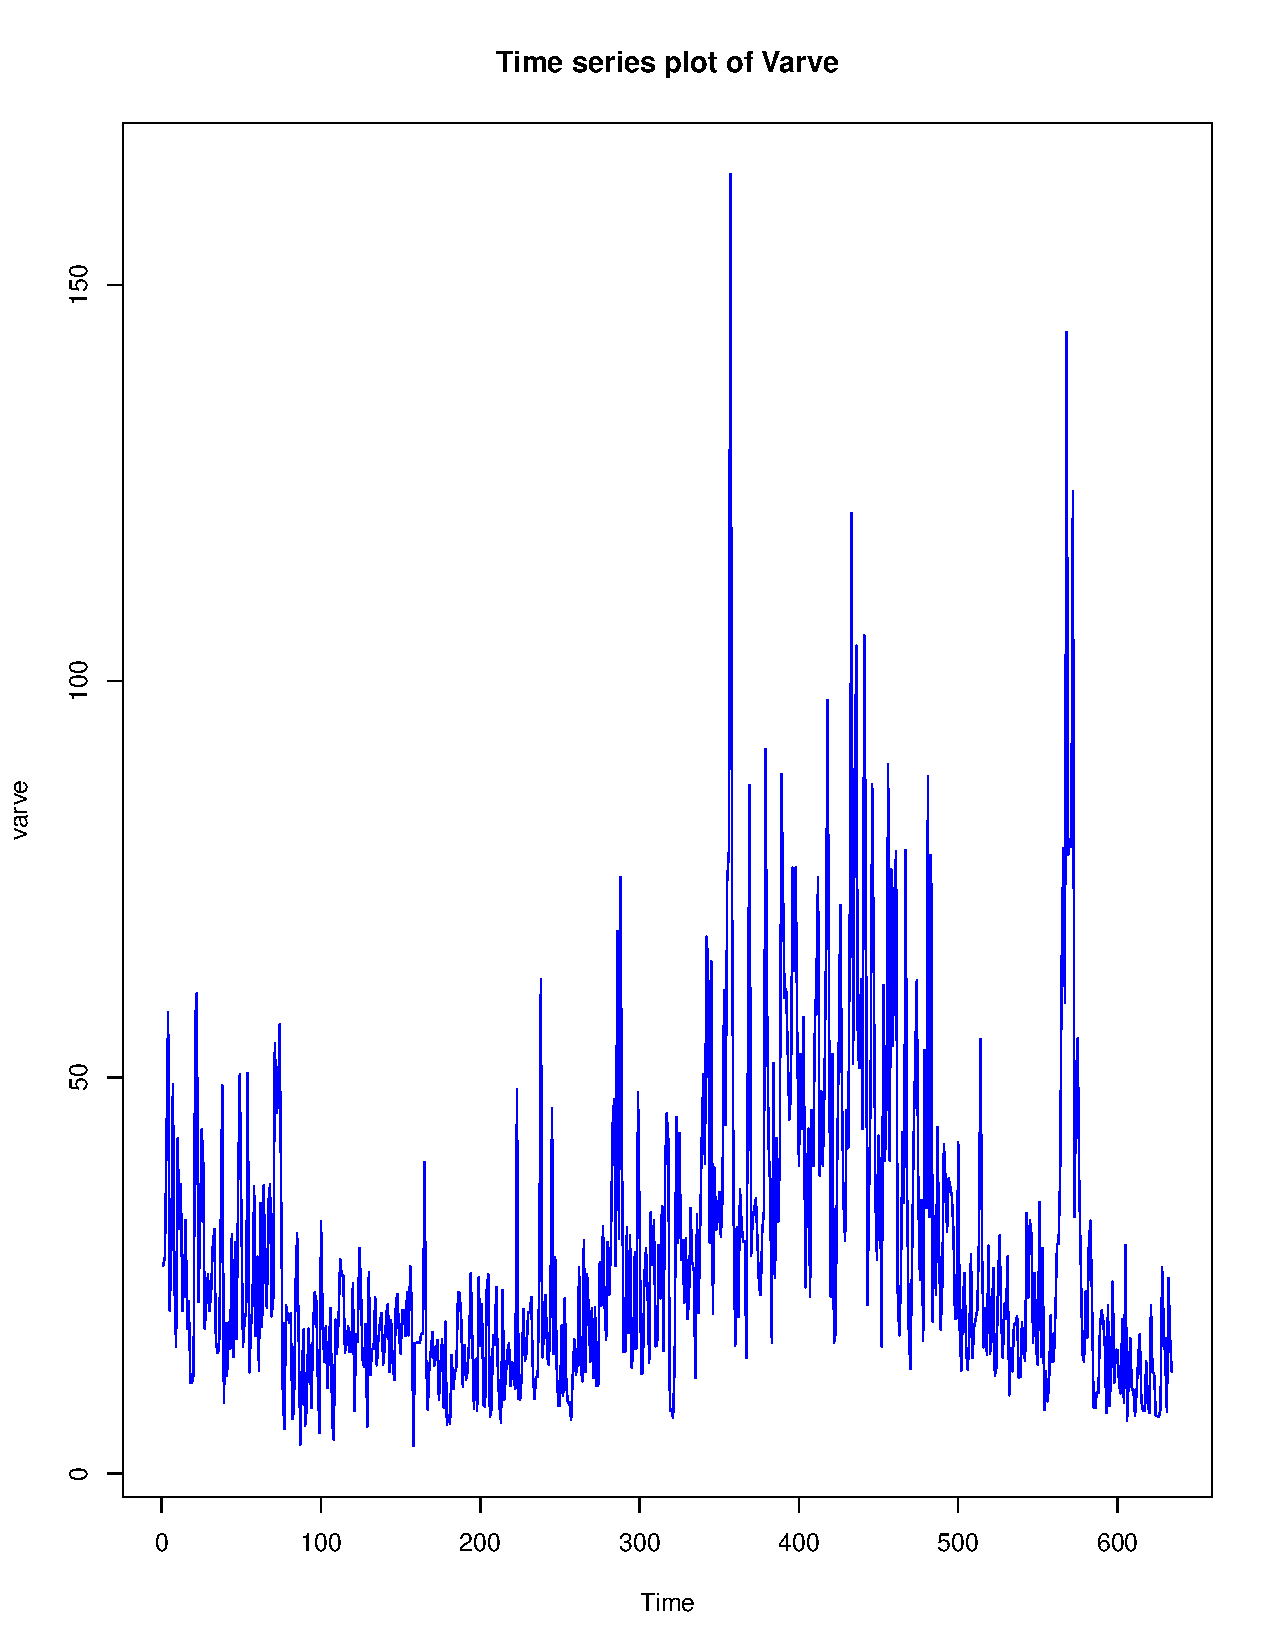
\includegraphics[width=0.9\textwidth]{Tsplot-varve}
	\caption{Time Series Plot, Varve }
	\label{fig:tsplot-varve}
\end{figure}

\begin{figure}
	\centering
	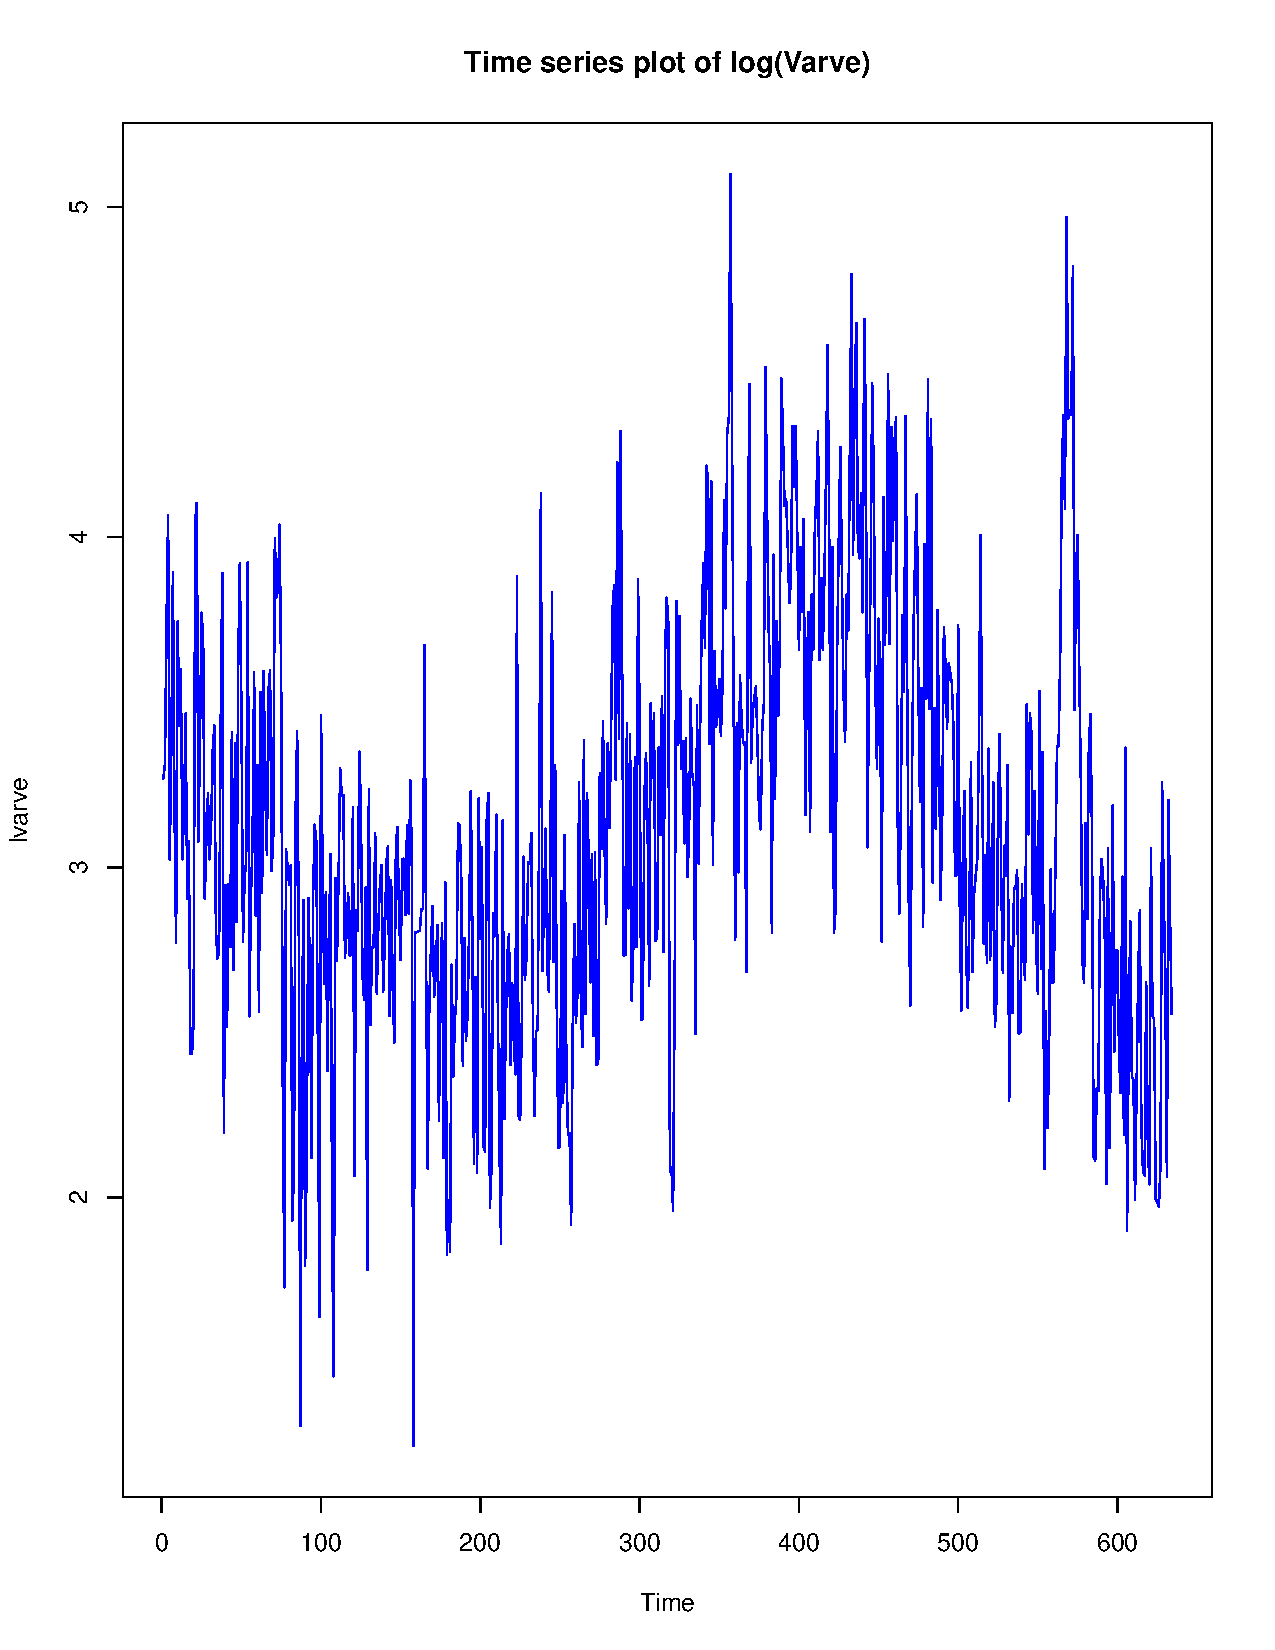
\includegraphics[width=0.9\textwidth]{TsPlot-lvarve}
	\caption{Time Series Plot, log(Varve) }
	\label{fig:tsplot-lvarve}
\end{figure}

\begin{figure}
	\centering
	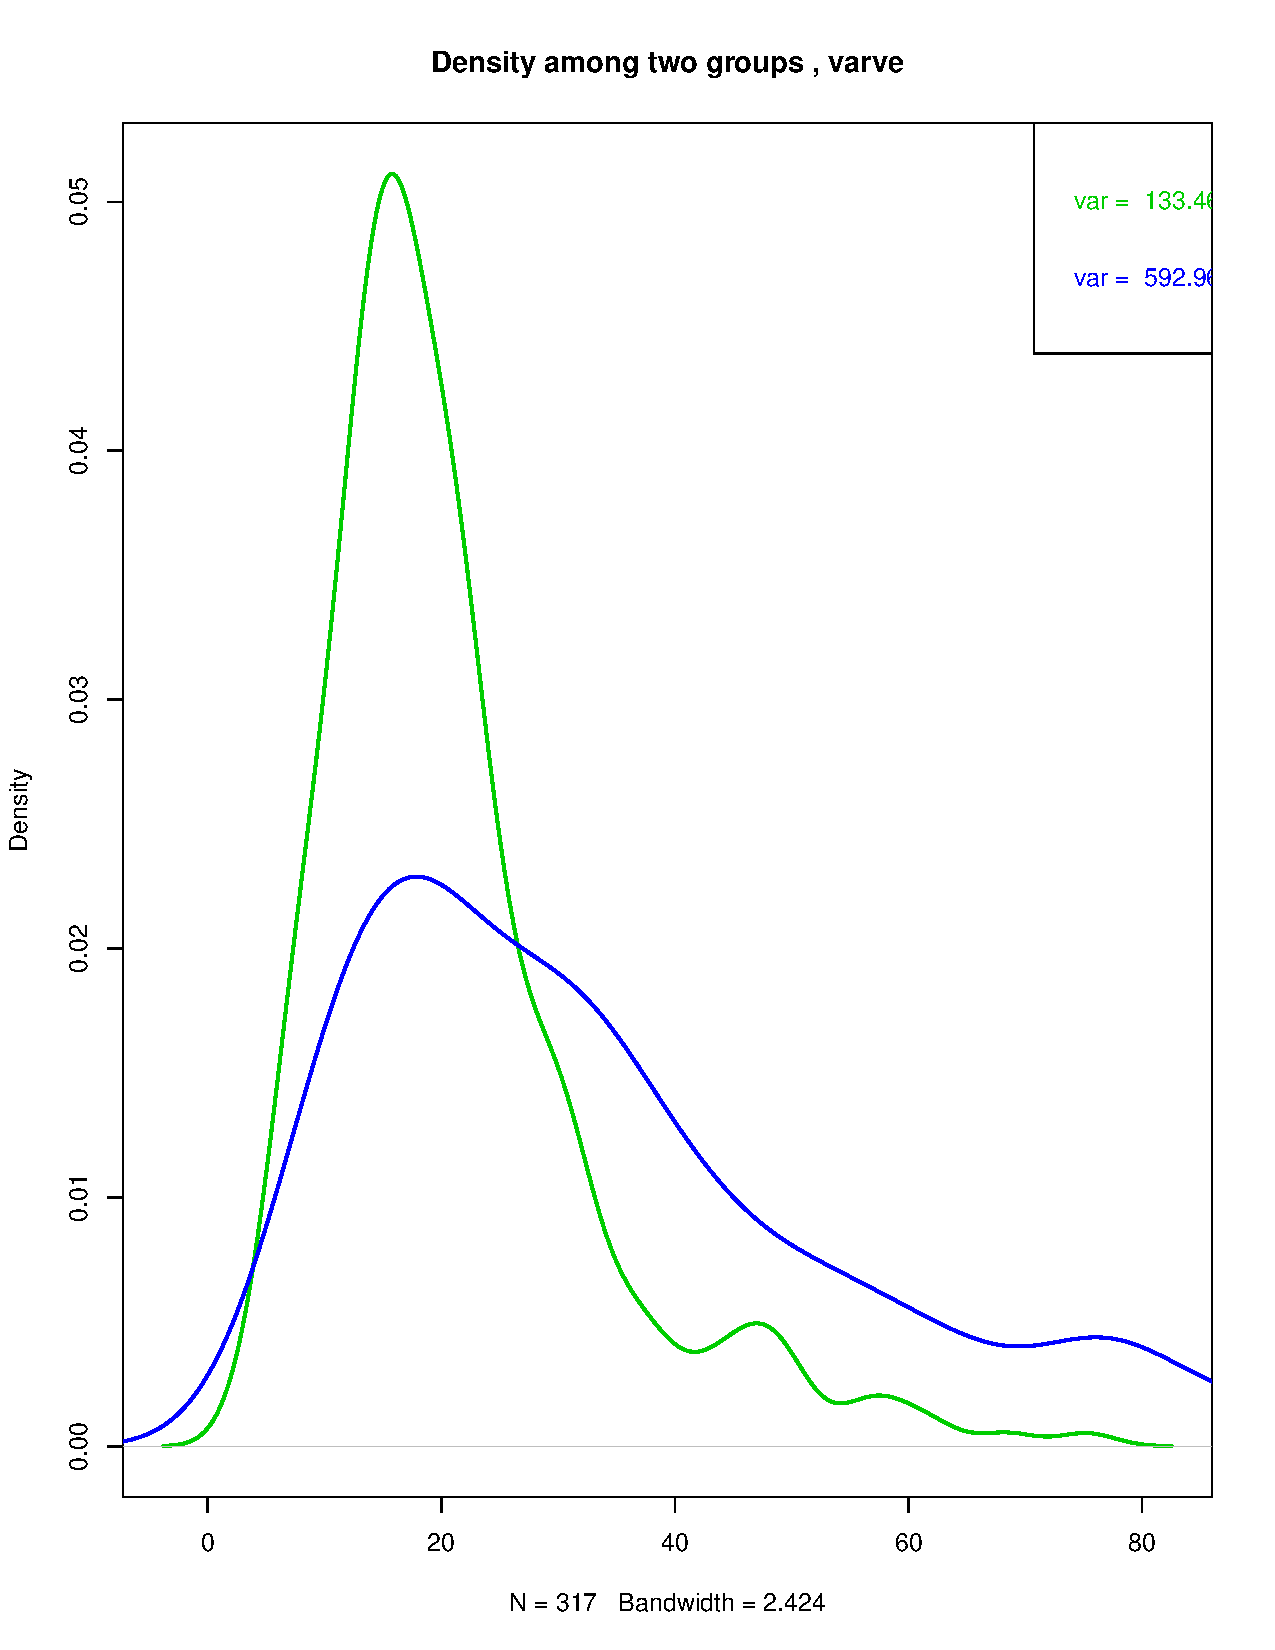
\includegraphics[width=0.9\textwidth]{DensityVarve}
	\caption{Density Plot, Varve }
	\label{fig:Density-lvarve-Plot}
\end{figure}

\begin{figure}
	\centering
	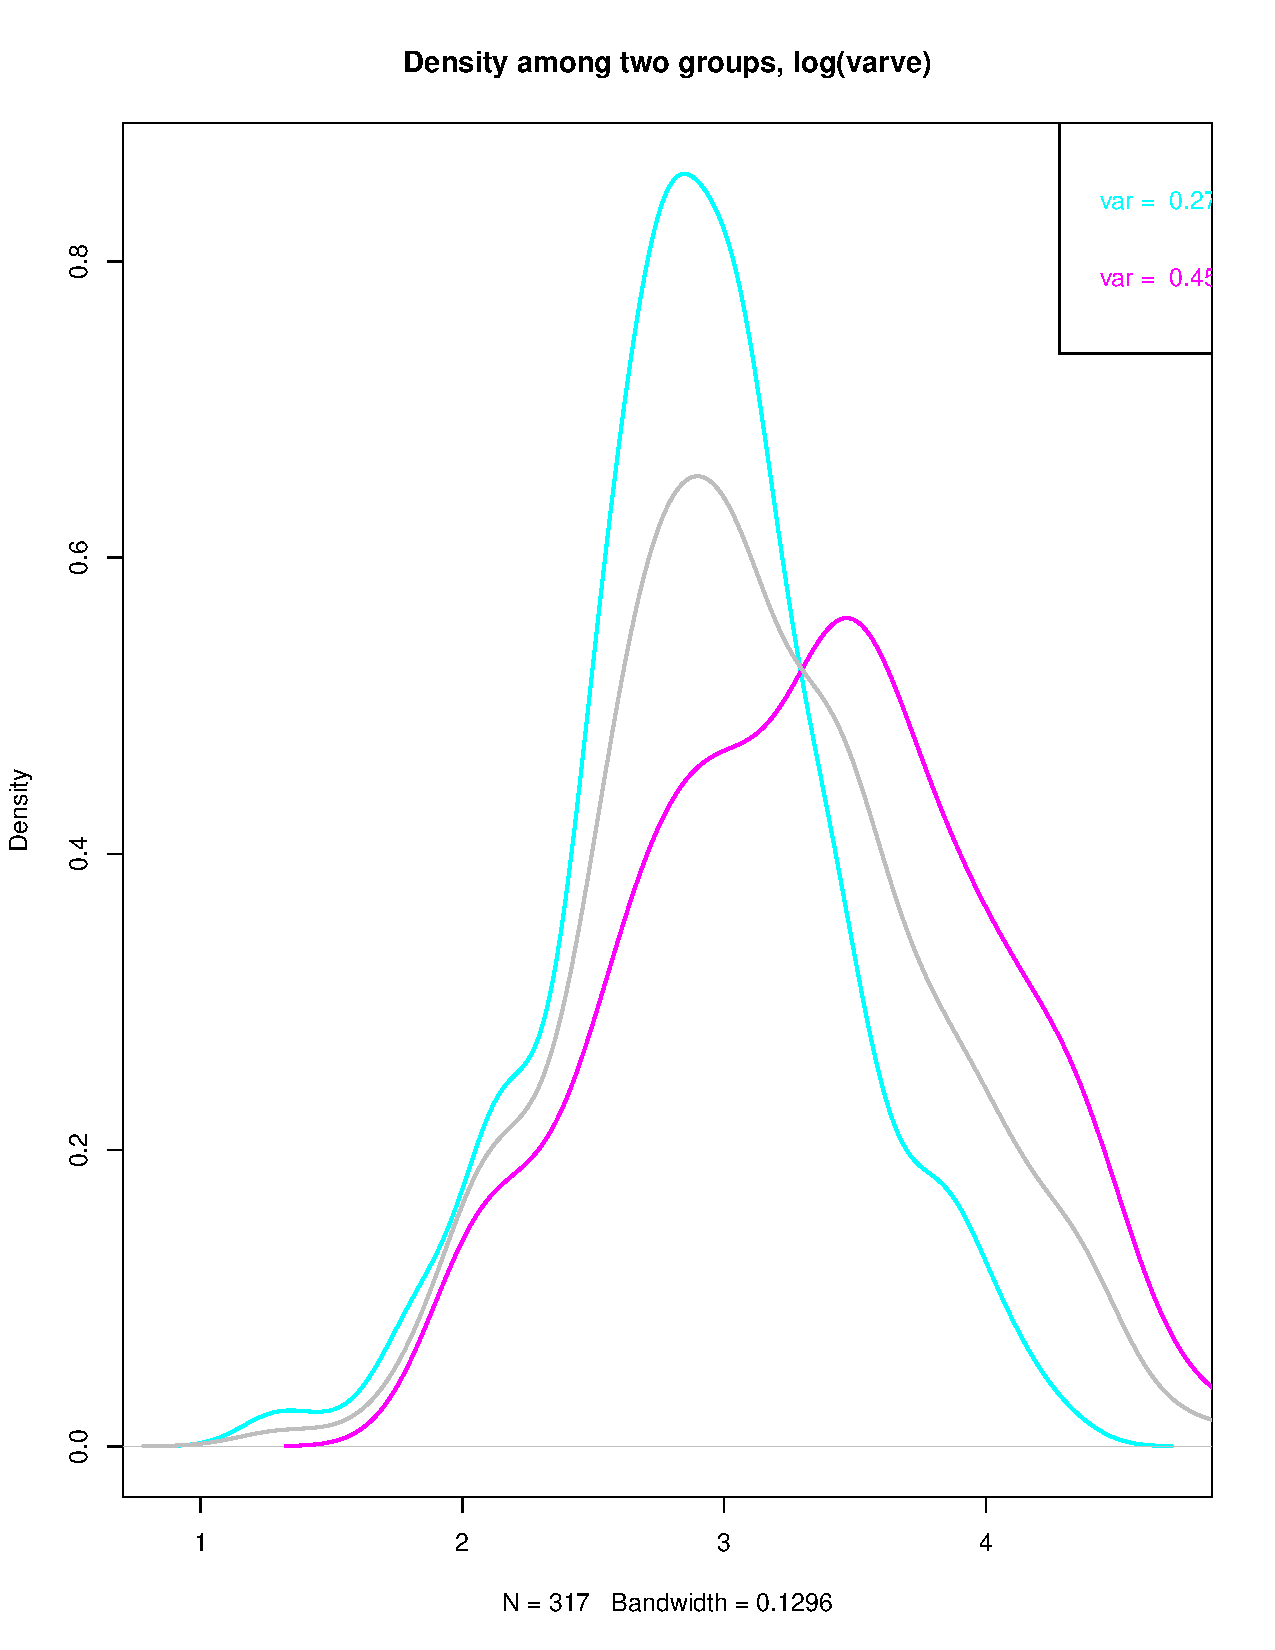
\includegraphics[width=0.9\textwidth]{Densitylvarve}
	\caption{Density Plot, log(Varve) }
	\label{fig:Density-varve-Plot}
\end{figure}


\begin{figure}
	\centering
	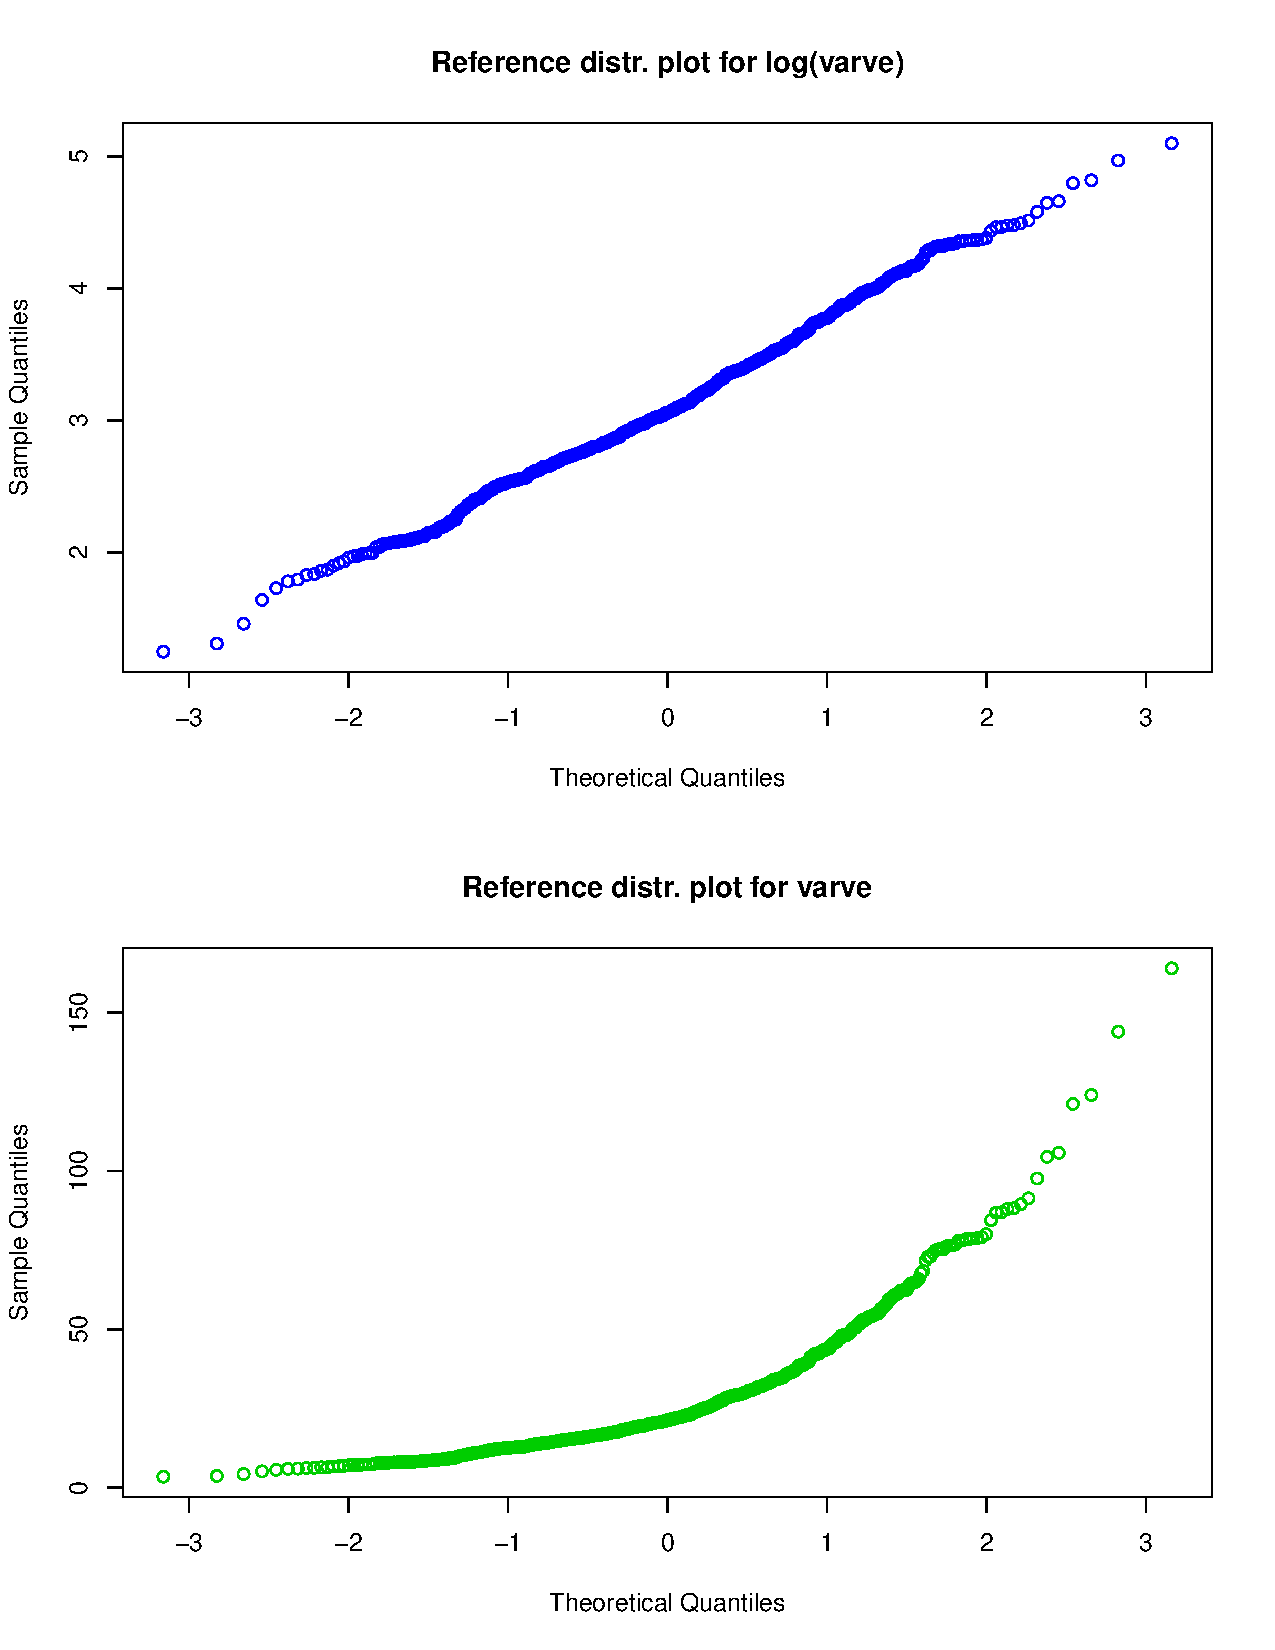
\includegraphics[width=0.9\textwidth]{QQPlot}
	\caption{Q-Q Plots before and after transformation }
	\label{fig:QQPlot}
\end{figure}

\subsection{b}

The series $y_t$ and $\log{y_t}$ are plotted in Figure \ref{fig:tsplot-varve} and Figure \ref{fig:tsplot-lvarve} respectively. 
Both these plots show evidence of the cyclical patterns as we saw in global temperature data. 

\subsection{c}

Sample ACF plot of Varve data as shown in Figure \ref{fig:acf} clearly indicates 
\begin{enumerate}
	\item  Cyclical patterns in the data.
	\item  Dependency i.e. auto-correlation of higher order lags.. 
 
\end{enumerate}


\begin{figure}
	\centering
	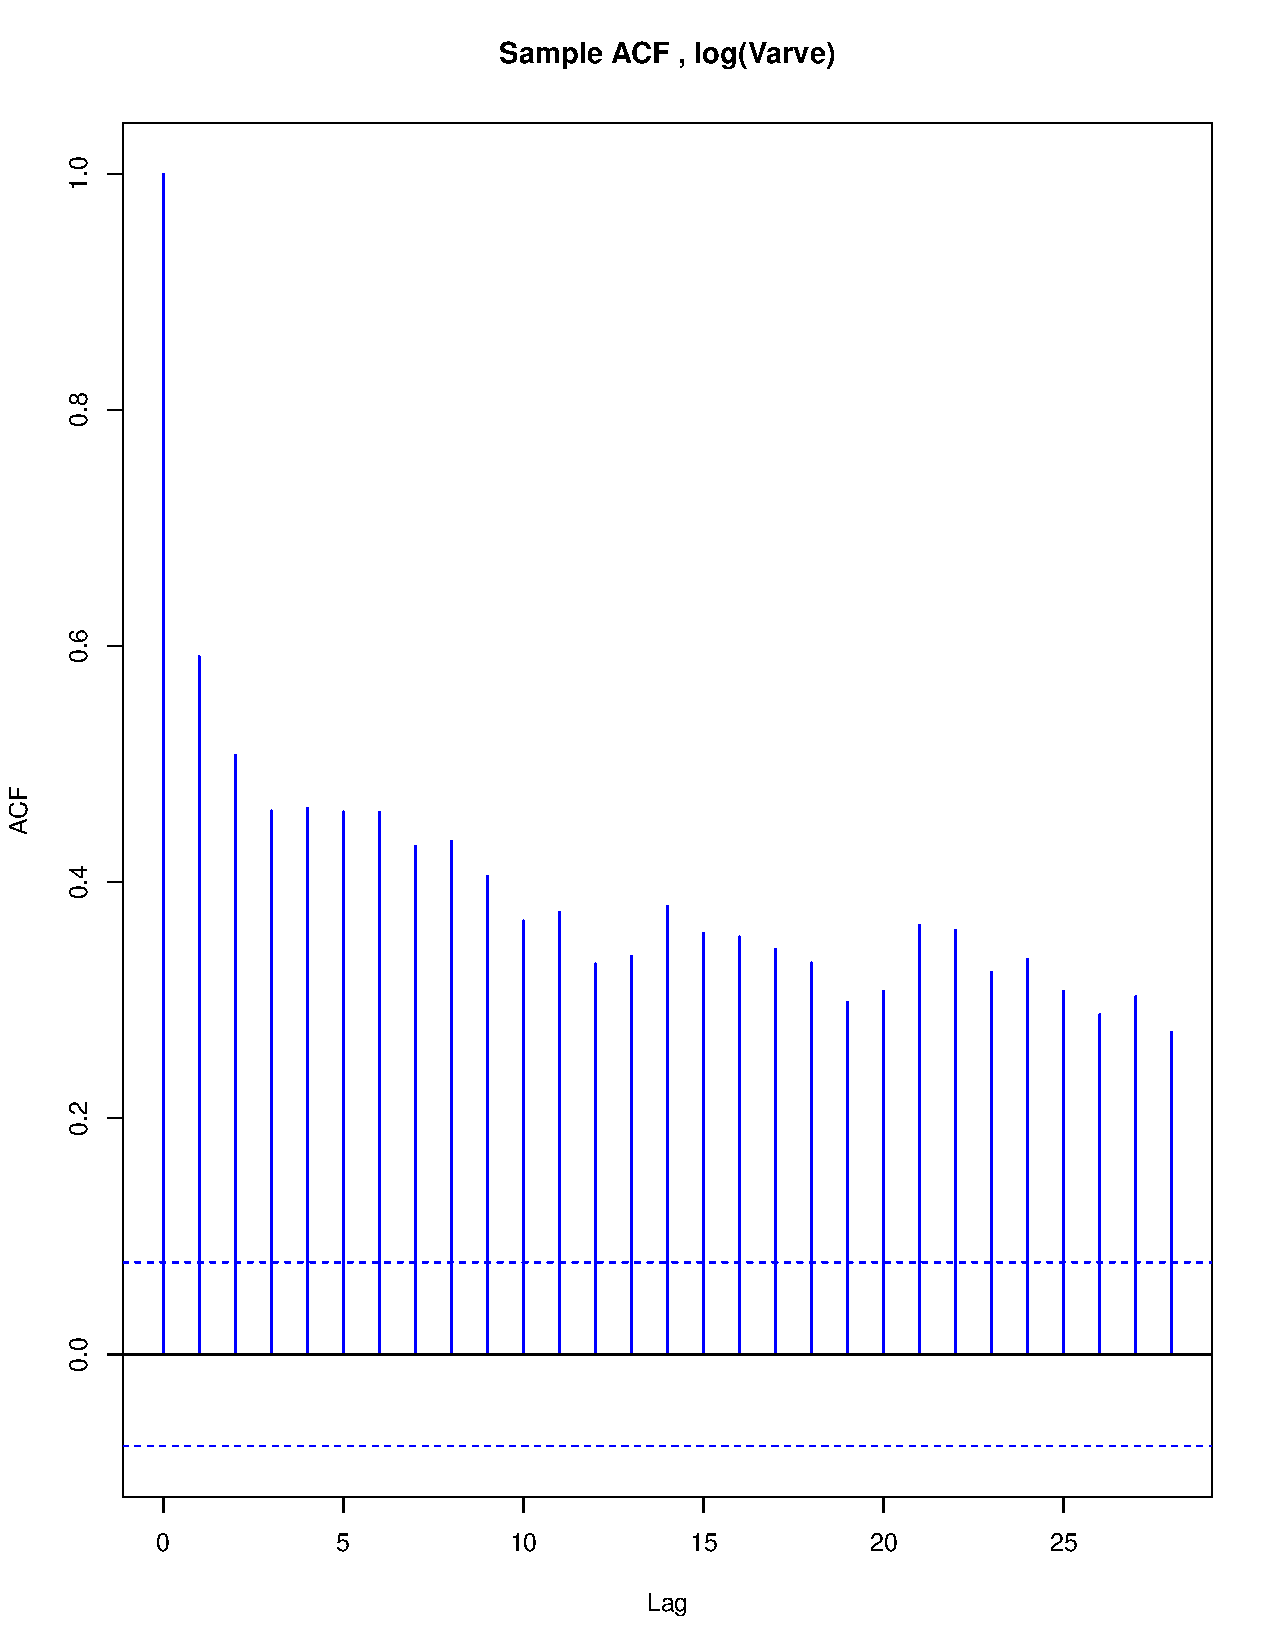
\includegraphics[width=0.9\textwidth]{SampleACF-lVarve}
	\caption{Sample ACF, log(Varve) Data }
	\label{fig:acf}
\end{figure}

\newpage
\subsection{d}

Sample ACF plot and First order differencing of Varve data as shown in Figure \ref{fig:acf-diff} and Figure \ref{fig:ts-diff} respectively. Figure \ref{fig:ts-diff} also has a smoothed Lowess curve overlayed . Both these figures provide visual support that
\begin{enumerate}
	\item  Any trend or cyclical pattern has been removed from the series.
	\item  Smoothed curve shows that the expected value from the sample , does not vary with the mean.
	\item  Sample Acf, does not detect higher order lag. 
	\item  Variance of the data has been controlled and does not vary with either time or lag. 
	\item  The data points look coming from $i.i.d$ distribution with a constant variance
	
\end{enumerate}
All of the above indicates that the Varve data set has been reduced to a stationary series now.


\begin{figure}
	\centering
	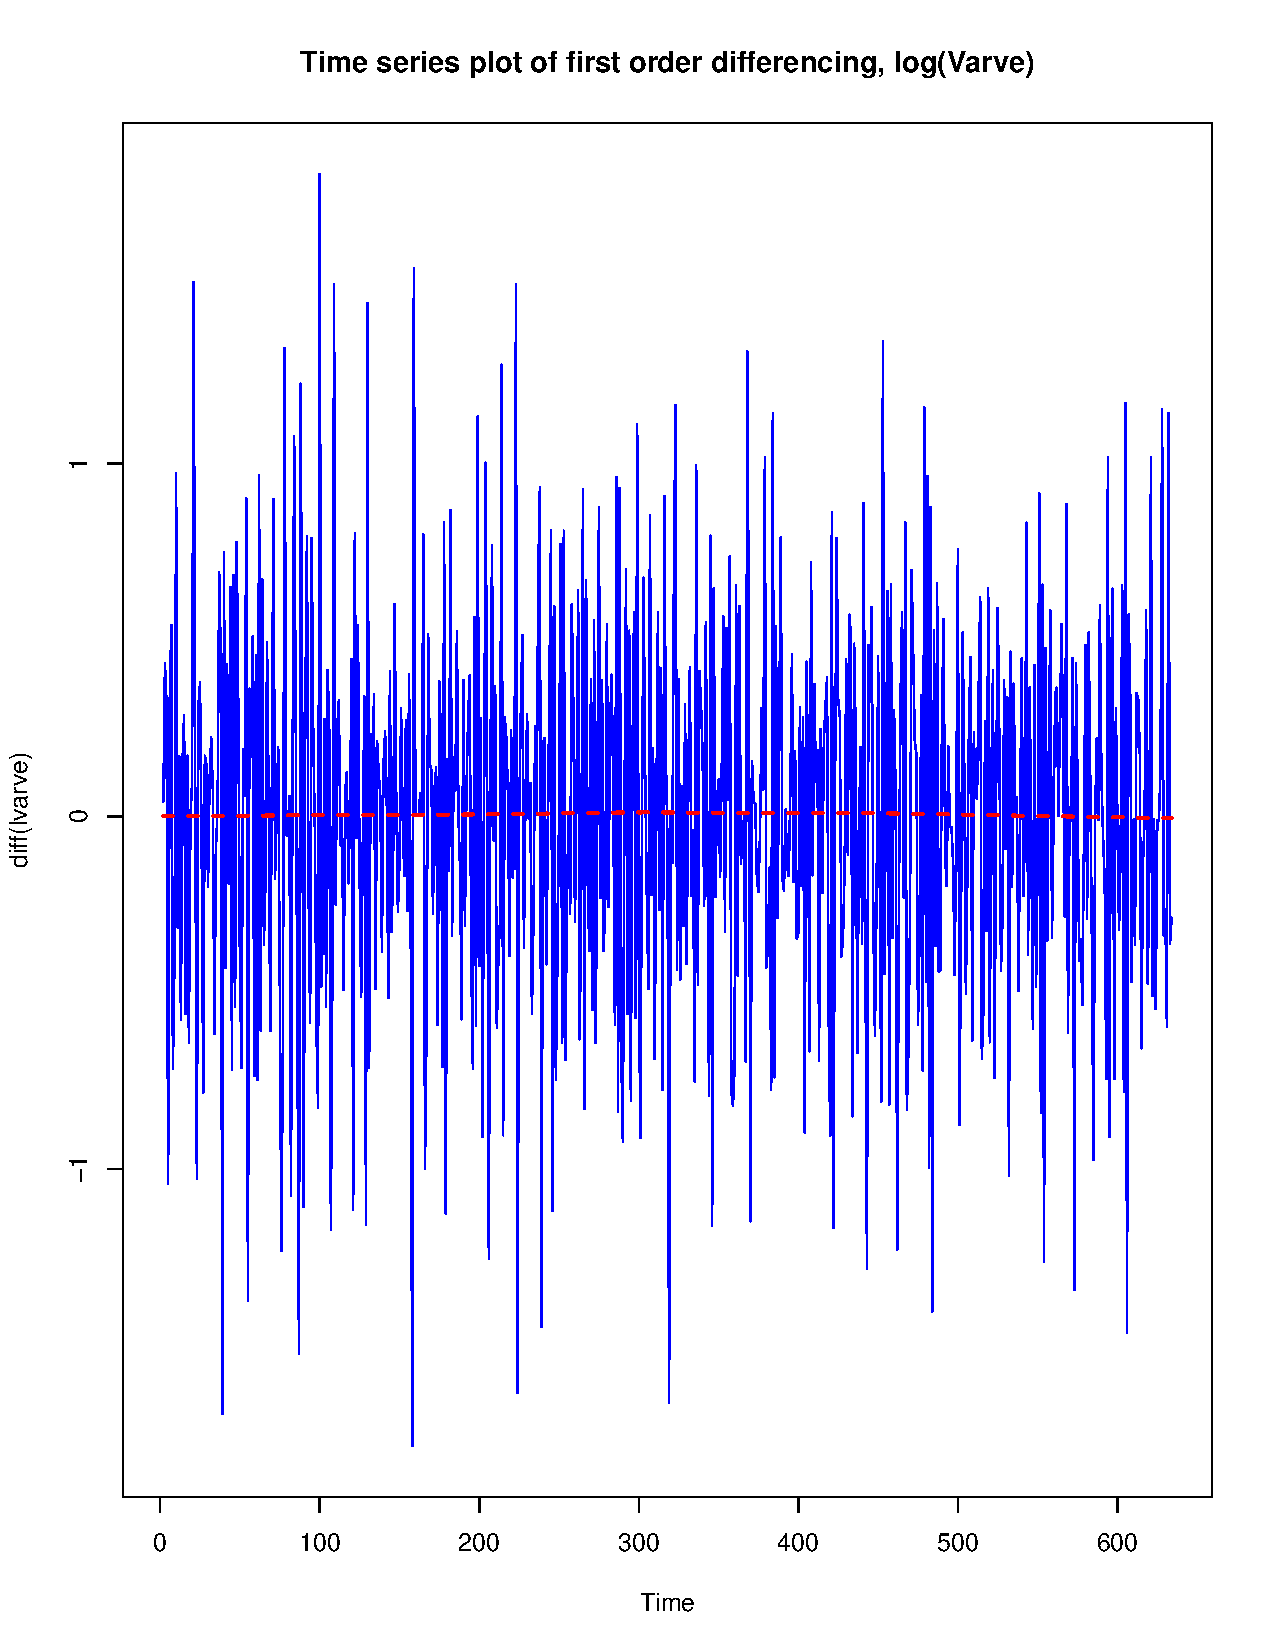
\includegraphics[width=0.9\textwidth]{DTSDiff}
	\caption{Time Series, 1st Order Differencing, log(Varve) Data }
	\label{fig:ts-diff}
\end{figure}

\begin{figure}
	\centering
	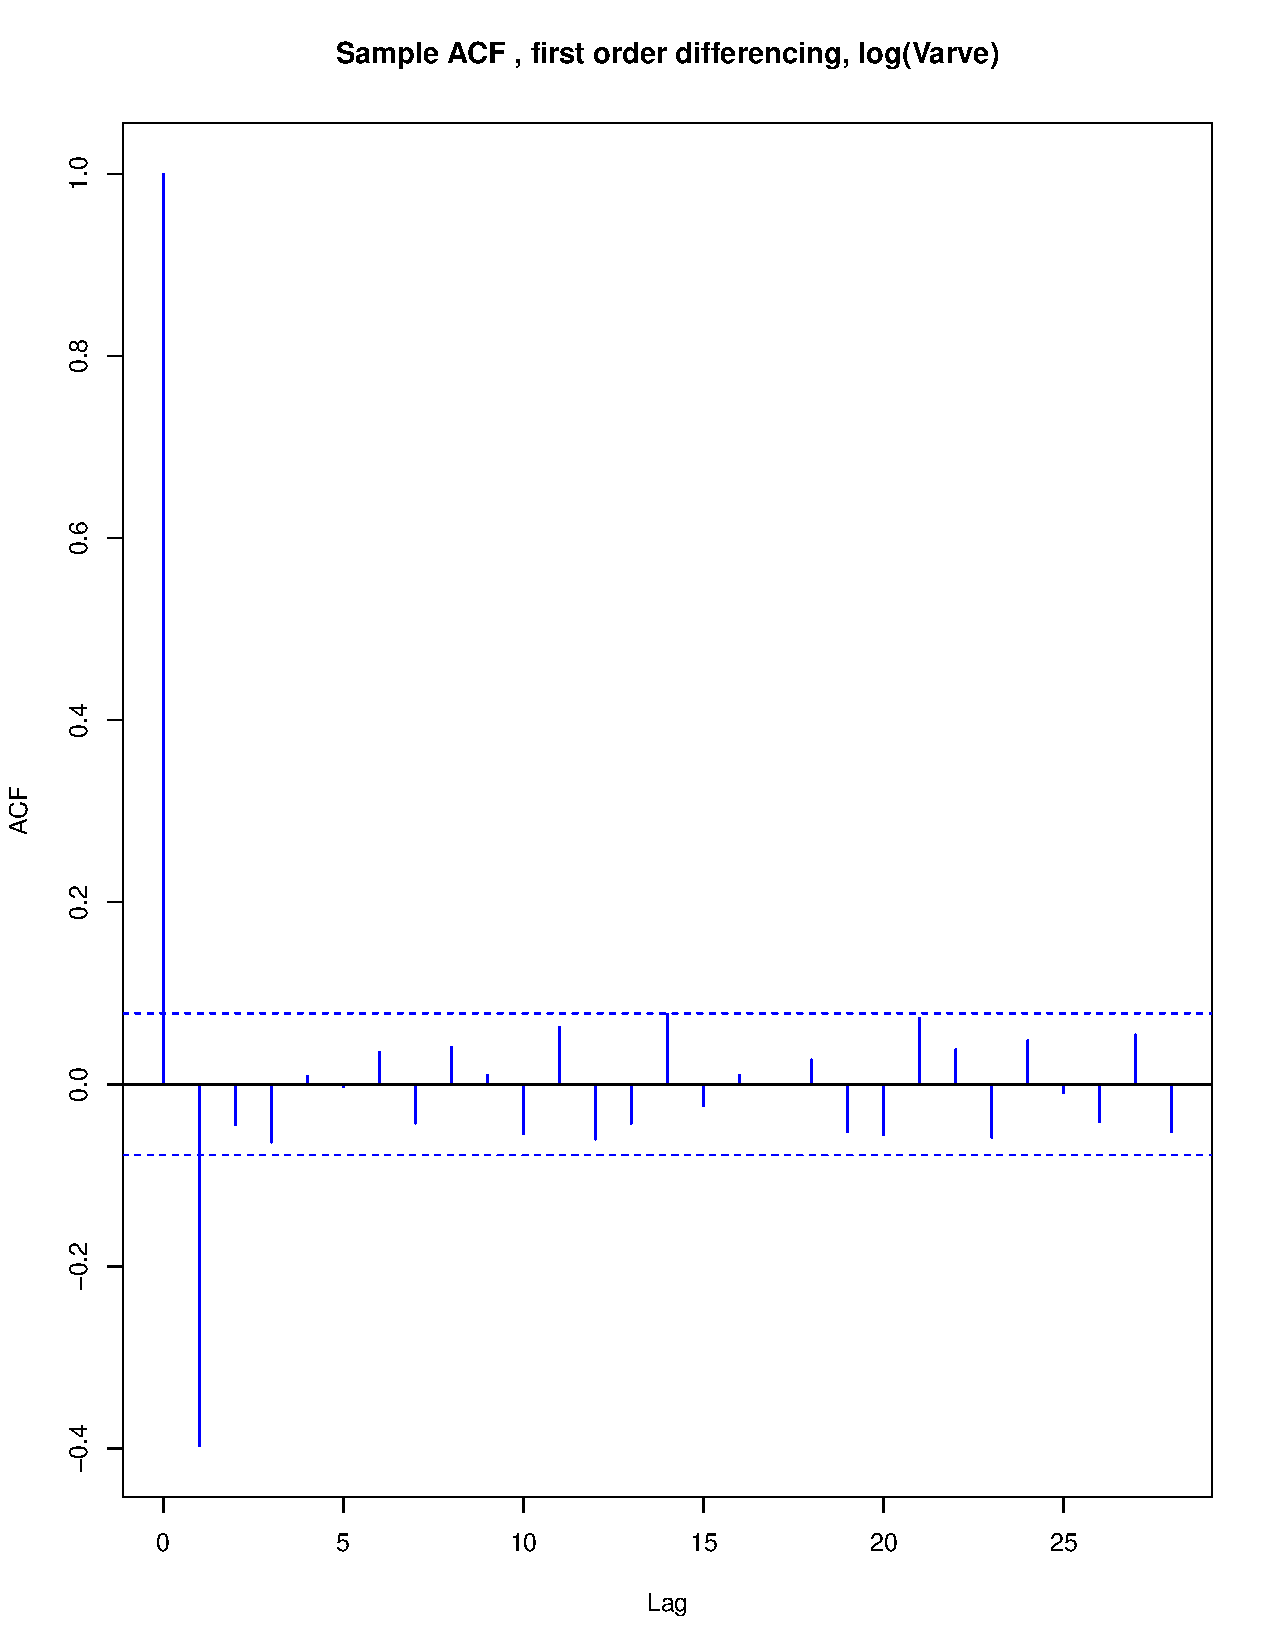
\includegraphics[width=0.9\textwidth]{ACF-Diff}
	\caption{Sample ACF, 1st Order Differencing, log(Varve) Data }
	\label{fig:acf-diff}
\end{figure}

\end{document}